The preceding chapters described the theory and algorithms of reinforcement learning. This chapter looks at where reinforcement learning actually survives contact with production systems, actual physical processes, marketplaces, and manufacturing. If we set aside game-engines, language-model post-training, and robotics, which are well covered elsewhere (\citep{Shao2019VideoGamesSurvey,Kaufmann2023RLHFSurvey,Ibarz2021robot,Tang2024RoboticsSurvey}) the cases of field applications of reinforcement learning are quite few and even fewer with adequete documentation. This chapter covers a few well documented cases so we can find out what might enable business applications of reinforcement learning. 

There cases come from recommendation engines, programmatic bidding, marketplace dispatch, inventory management, video encoding, and chip design; RLHF is included as a training-time success case, not as evidence that ordinary business control problems have been solved at comparable breadth. The gap between academic application and publicly documented business impact is therefore quite large. Field systems where RL works, usually only give RL a narrow control surface, surround it with an ecosystem of historical and live logs that track older and current policies and counterfactual evaluation of said policies. There is, in short, a lot of infrastracture that is necessarily for business deployment of reinforcement learning. 

\begin{table}[t]
\centering
\footnotesize
\begin{tabular}{p{0.24\linewidth}p{0.66\linewidth}}
\toprule
Case & What the source establishes \\
\midrule
YouTube recommendations & Production top-$K$ candidate generation with REINFORCE and live YouTube experiments \citep{Chen2019YouTubeTopK}. \\
Meta notifications & Horizon-trained RL policies replaced supervised notification systems for some Facebook notifications \citep{Gauci2019Horizon}. \\
Taobao cold-start ranking & RL-LTV was deployed on Taobao for cold-start recommendation, with live A/B results \citep{Ji2021RLLTV}. \\
Meta production bidding & Offline RL optimized parameters of an existing production auto-bidding policy and was A/B tested at scale \citep{Korenkevych2023MetaBidding}. \\
Alibaba sponsored-search RTB & Robust-MDP bidding control was deployed and tested in Alibaba's search auction platform \citep{Zhao2018SponsoredSearchRTB}. \\
DiDi dispatch & RL dispatch was A/B tested in multiple cities and launched as primary dispatch in a major market \citep{SadeghiEshkevari2022DiDiScalable}. \\
DeepStock inventory & DRL with inventory-policy regularization was rolled out across Tmall SKU-warehouse replenishment \citep{Xie2026DeepStock}. \\
MuZero-RC video encoding & MuZero-RC controlled VP9 rate control on part of YouTube live traffic \citep{Mandhane2022MuZeroRC,DeepMind2022MuZeroRCPost}. \\
AlphaChip floorplanning & RL-generated layouts were used in Google TPU and other shipped chip designs, a design artifact rather than a runtime controller \citep{Mirhoseini2021GraphPlacement,GoldieMirhoseini2024AlphaChipPost}. \\
InstructGPT RLHF & PPO against a learned reward model shaped deployed language-model behavior, training-time RL rather than inference-time control \citep{ouyang2022training}. \\
BCOOLER HVAC & RL produced live supervisory-control recommendations at two commercial buildings, field trials without broad rollout \citep{Luo2022BCOOLER}. \\
Tmall pricing, hotel revenue management & Real field experiments controlled prices or revenue-management decisions, without broad rollout evidence \citep{Liu2019,Chen2023hotelrl}. \\
Financial execution, RTB simulator, inventory benchmark & Real data or benchmark evidence without public proof of live deployed control \citep{Nevmyvaka2006execution,Wu2018rtb,Gijsbrechts2022inventory}. \\
\bottomrule
\end{tabular}
\caption{Public primary-source evidence for field RL cases.}
\label{tab:field_case_inventory}
\end{table}

\subsection{Digital Traffic: Recommendations and Notifications}

\subsubsection{YouTube recommendations}
\label{sec:youtube_topk}
YouTube's top-$K$ recommender is the cleanest public case of a formal reinforcement-learning result placed inside a production system that was already sophisticated \citep{Chen2019YouTubeTopK}. The learned policy did not run the whole recommender. It was one of several systems that nominate a short list of candidate videos, and a separate model then scored that pooled list and built the page the user saw.\footnote{The paper calls a nominating system a candidate generator and the scoring model a ranker, and the learned policy here was one candidate generator among many. Its metric of record is what the paper names ViewTime, the time users spent watching videos on YouTube.} The surface it controlled was narrow, changing which videos entered the ranking funnel rather than the final page, and it was judged on the time users spent watching. That narrow and well-instrumented surface is what makes the case credible as field evidence rather than a demonstration.

The starting point is a formal object this monograph has already built. Recall the policy-gradient (REINFORCE) update of Section~\ref{section:rl_algorithms}. When a policy $\pi_\theta$ learns from its own trajectories, each logged choice is nudged along
\begin{equation}
\label{eq:yt_reinforce}
\nabla_\theta J(\theta) = \mathbb{E}_{\tau \sim \pi_\theta}\!\left[\sum_{t \geq 0} R_t\, \nabla_\theta \log \pi_\theta(a_t \mid s_t)\right],
\end{equation}
where $R_t = \sum_{t' \geq t} \gamma^{t'-t} r(s_{t'}, a_{t'})$ is the discounted return from time $t$. In the recommender the state $s$ is a recurrent summary of the user's watch history, the action $a$ is one video from a catalog of order $10^6$, and the policy is a softmax over videos, $\pi_\theta(a \mid s) \propto \exp(s^\top v_a / T)$ with temperature $T$. Two facts about the production setting force two small and self-contained changes to this update, and those two changes are the paper's contribution.

The first fact is that observing a reward means showing a real video to a real user, so the policy cannot generate fresh trajectories of its own. It learns instead from choices logged by earlier and parallel recommenders, a behavior policy $\beta$, and the standard fix reweights each logged choice by the importance ratio $\pi_\theta(a \mid s) / \beta(a \mid s)$ in place of the plain gradient.\footnote{The behavior policy $\beta$ is not logged directly, since some logging agents are deterministic or outside YouTube's control, so it is estimated by a second softmax head that shares the recurrent user state with the main policy and has its gradient blocked from that state. The estimated ratio is then capped at $c = e^3$ to bound its variance. Other chapters write $\pi_b$ for this logging policy; here $\beta$ follows the off-policy literature and clashes with nothing, since the discount is $\gamma$ and the softmax temperature is $T$.} The second fact is that the product returns a set of videos rather than one. Drawing $K$ items independently from $\pi_\theta$ and removing duplicates, an item's chance of appearing at least once is its inclusion probability
\begin{equation}
\label{eq:yt_alpha}
\alpha_\theta(a \mid s) = 1 - \big(1 - \pi_\theta(a \mid s)\big)^K .
\end{equation}
Optimizing this inclusion probability rather than the single best choice multiplies the off-policy update by one extra factor, giving the paper's result
\begin{equation}
\label{eq:yt_topk}
\boxed{\nabla_\theta J_K(\theta) \approx \mathbb{E}_{s \sim d^\beta,\, a \sim \beta}\!\left[ \frac{\pi_\theta(a \mid s)}{\beta(a \mid s)}\, \lambda_K(s,a)\, R(s,a)\, \nabla_\theta \log \pi_\theta(a \mid s) \right]}
\end{equation}
with the top-$K$ multiplier $\lambda_K(s,a) = K\big(1 - \pi_\theta(a \mid s)\big)^{K-1}$.\footnote{The multiplier is the derivative $\partial \alpha_\theta / \partial \pi_\theta$ of the inclusion probability, so the top-$K$ update is a chain-rule consequence of optimizing $\alpha_\theta$. The inclusion probability reaches one half at $\pi_\theta(a \mid s) = 1 - 2^{-1/K} \approx (\log 2)/K$, so an item needs probability only of order $1/K$, not near one, to have an even chance of appearing in the slate.}

The two changes read cleanly. The ratio $\pi_\theta / \beta$ removes the behavior policy's selection bias, undoing the tendency of an uncorrected learner to keep recommending whatever was already shown most, a rich-get-richer effect. The multiplier $\lambda_K$ turns a top-1 learner into a top-$K$ one. It is close to $K$ for a video the policy currently rates as unlikely, so a promising but under-exposed item is pushed up hard, and close to zero for a video already almost certain to appear, so the policy stops spending probability on making one item a lock and funds the second and third candidates instead. At $K = 1$ the multiplier is one and the ordinary correction returns.

Two caveats travel with the result. The first-order estimator that is actually deployed is biased. It corrects which video was chosen in a logged state, but not how often the new policy would reach that state, nor the later choices that produced the return, so its expectation is not the true policy gradient.\footnote{A genuinely unbiased off-policy gradient reweights the whole trajectory by the product $W(\tau) = \prod_t \pi_\theta(a_t \mid s_t) / \beta(a_t \mid s_t)$, whose expectation under $\beta$ equals the on-policy gradient because the initial-state and transition factors cancel. That product is a chain of ratios whose variance explodes at YouTube's scale, and the estimated $\beta$ compounds the error, so the paper drops the state-visitation ratio $d^\pi/d^\beta$ and the future-action ratios and keeps only the current-action term. Bias here means the estimator's expectation differs from $\nabla_\theta J(\theta)$, not merely that it is noisy; \citet{Chen2019YouTubeTopK} invoke a bound of Achiam et al.\ on the resulting gap in terms of the total-variation distance between $\pi_\theta$ and $\beta$.} It also needs the logging policy to have placed some probability on every video the new policy wants to try, since no reweighting recovers an outcome that was never observed.\footnote{This condition, that $\pi_\theta(a \mid s) > 0$ implies $\beta(a \mid s) > 0$, is the standard common-support requirement of off-policy learning rather than the paper's own language. \citet{Chen2019YouTubeTopK} speak instead of sparse data over an action space in the millions, and of large or noisy importance ratios, as the sources of instability.} And the reduction to a per-item update rests on two slate assumptions.\footnote{The reduction assumes at most one item in the returned set earns reward and that an item's value does not depend on the others shown, which sets aside within-slate competition, complementarity, position effects, and multiple clicks.} These are the compromises the method accepts to run at scale.

Do the two changes actually change the recommendations? In the paper's two controlled simulations they do, visibly. In the first, where the logging policy over-shows the least-rewarded items, an uncorrected learner inherits that skew and misses the best item, and adding the off-policy correction recovers it. In the second, with a uniform logging policy and one clearly best item, the standard correction swings to the opposite failure and puts almost all of its mass on that single item, while the top-$K$ correction keeps real mass on the second-best as well.\footnote{The first simulation has ten items with reward $r(a_i) = i$ and a behavior policy $\beta(a_i) = (11-i)/55$ skewed toward the least-rewarded items; without correction the learned policy converges to the reward-weighted behavior $\propto r \cdot \beta$, a mound over the middle items that misses the optimum, and with the off-policy correction it recovers the optimal item (Figure 2 of the source). The second simulation gives one item reward $10$, the next reward $9$, and the rest reward $1$ under a uniform behavior policy; the standard correction collapses onto the single best item, $\pi(a_1) \approx 1$, while the top-2 correction keeps significant mass on the second-best, roughly a $0.6$ and $0.4$ split read from Figure 3 of the source, which prints no numbers.} In the live system the clearest direct evidence is that adding the off-policy correction raised nominations of videos outside the historically top ranks by nearly a factor of three, a genuine change in the candidate sets, while the top-$K$ correction added a lift of 0.85 percent in watch time over the previous model.\footnote{The threefold change is the no-correction-versus-standard-correction comparison (Figure 4 of the source, a live A/B test), not a top-1-versus-top-$K$ result. For top-1 versus top-$K$ the paper publishes only watch time and the number of videos viewed, with no candidate-overlap, catalog-coverage, entropy, or diversity statistic, and the candidate sets are re-ranked downstream before display.} The premise underneath all of this is dynamic, that today's recommendation shapes tomorrow's user state, yet the paper does not isolate that this sequential effect is what paid off, so the demonstrated gains are the exposure and slate-shape changes just described rather than measured dynamic preference formation.\footnote{The model retrained continuously over calendar time, but the paper shows no training or cumulative-reward curve and no early-versus-late checkpoint comparison; Figure 5 of the source is a five-day A/B effect plot, not a learning curve. There is no ablation of the discount, and the simulations are explicitly stateless, so whether the sequential structure itself contributed is left open.}

Table~\ref{tab:youtube_topk_live} collects the reported live effects, which are sub-percent movements in watch time\footnote{Read against a standard metric hierarchy, the north-star is watch time and the secondary engagement metric is the number of videos viewed. The algorithmic diagnostic is the distribution of nominations by rank; the exploration evidence is a $0.07$ percent watch-time gain from a five-percent stochastic-exploration traffic slice at equal data volume; the operational facts are continuous training with a data lag under 24 hours, a reward horizon of 4 to 10 hours, and serving by sampled softmax at training time and approximate nearest-neighbor retrieval over the learned embeddings at serving time. Explicit safety, quality, or diversity guardrails are not reported.} measured as component tests against evolving controls rather than a replacement of YouTube's recommender.\footnote{The system improved in sequence, from a reward-only policy gradient to the standard off-policy correction to the top-$K$ correction, and each stage became the control for the next, so the effects are not additive. Across $K \in \{1, 2, 16, 32\}$ the production setting was $K = 16$, with $K = 1$ losing $0.66$ percent watch time, $K = 2$ losing $0.35$ percent, and $K = 32$ matching $K = 16$; a later followup with $K = 8$ gave a mild $0.15$ percent gain but was not adopted.} The lesson is the one this chapter keeps finding. An established formal result, the score-function policy gradient of Section~\ref{section:rl_algorithms},\footnote{A value-based alternative would fit an action-value $Q_\phi(s,a) = h_\phi(s)^\top v_a$, train it toward a Double-DQN target, and serve the top $K$ by nearest-neighbor search over $Q$. Q-learning is naturally off-policy, but its Bellman target maximizes over millions of actions, most with little logged support. \citet{Chen2019YouTubeTopK} prefer policy gradients because value-based methods can be unstable under nonlinear function approximation, need heavy tuning, and lack established policy-convergence guarantees, and they report no empirical Q-learning comparison.} carried into a live system with two disciplined modifications and hard variance control, buys a small, real, well-measured gain.\footnote{The gain is measured against the immediately preceding production model, not against the prior supervised recommender, contextual bandits, the full ensemble of candidate generators, or the final ranker. The live experiments carry no random-policy lower bound and no oracle upper bound, and the optimal policy appears only in the stateless simulation.} The price is a set of visible compromises,\footnote{The obstacles the paper foregrounds, in the order it emphasizes them, are logged-policy bias and thin coverage, the scale and sparsity of a catalog in the millions, the mismatch between a top-1 policy gradient and a top-$K$ product, the variance of the importance weights, limited exploration that must not harm users, and batched, nonstationary learning.} a deliberately biased estimator, capped importance weights, and a control surface kept narrow on purpose, and paying it is what let the method reach production.

\begin{table}[t]
\centering
\small
\begin{tabularx}{\textwidth}{@{}>{\raggedright\arraybackslash}p{0.27\textwidth}>{\raggedright\arraybackslash}X>{\raggedright\arraybackslash}p{0.20\textwidth}@{}}
\toprule
Intervention & Live comparison & Reported effect \\
\midrule
Exploratory data & Train with a 5\% stochastic-policy traffic slice rather than only deterministic-policy logs & +0.07\% ViewTime \\
Standard off-policy correction & Weight logged examples by learned behavior-policy importance ratios & +0.53\% videos viewed; no significant ViewTime change \\
Top-$K$ off-policy correction & Train the production candidate generator with $K=16$ top-$K$ correction & +0.85\% ViewTime; -0.16\% videos viewed \\
Top-1 ablation & Set $K=1$, reducing the correction toward the standard top-1 case, versus production $K=16$ & -0.66\% ViewTime \\
Uncapped-weight regression & Loosen the importance-weight cap from $e^3$ to $e^5$ & -0.52\% ViewTime \\
\bottomrule
\end{tabularx}
\caption{Live YouTube experiments reported by \citet{Chen2019YouTubeTopK}. Effects are relative to the relevant control model in each sequential experiment, so rows should be read as component tests rather than additive gains.}
\label{tab:youtube_topk_live}
\end{table}

\subsubsection{Meta notifications}
Horizon, Facebook's applied RL platform, gives a second digital-traffic case \citep{Gauci2019Horizon}. The strongest sourced example is notification control: for a notification candidate, the policy chooses whether to send or drop, using person and notification features and a reward that combines activity, meaningful interaction, and a penalty for sending. The decision process is the sequence of notification candidates for one person, an episodic formulation whose finite horizon spans the multiple weeks of training data, with discounted accumulated reward over the discrete send-or-drop pair. Horizon's surrounding infrastructure matters as much as the DQN-style policy. The paper emphasizes preprocessing, distributed training, optimized serving, and counterfactual policy evaluation because online errors affect real people.\footnote{The Horizon paper also mentions Facebook 360 adaptive bitrate, but the sourced passage lacks enough public detail to classify it as confirmed production RL, so it is not counted as a core case.}

\subsubsection{Taobao cold-start recommendation}
\citet{Ji2021RLLTV} frame cold-start item recommendation on Taobao as an item-lifetime-value problem. The state is item-level history, including exposure, interaction, sale, and time features; the learned action contributes an RL score to a dual-rank system. The live evidence is a one-week Taobao A/B test beginning on January 26, 2021, with reported cold-start-item gains of 8.67\% in item page views and 18.03\% in gross merchandise value relative to the Vanilla-CTR baseline.

Operationally, RL-LTV runs at the item-day frequency rather than the request-serving frequency. User logs are aggregated by item and by day into item episodes, each a finite-horizon window of daily steps over the item's early lifetime, discounted at $\gamma=0.5$; the actor produces an LTV-oriented score $y_{\mathrm{rl}}$, and the critic estimates future item value. The online ranker keeps the conventional CTR score $y_{\mathrm{ctr}}$ and combines it with $y_{\mathrm{rl}}$ through a dual-rank module whose mixing weight is bounded in the experiment. The serving system therefore receives a ranking score, while the RL training loop updates from daily item histories.

The formal action space is broader than the live control surface. The paper's action includes both an RL score and a price-like component, but the source notes that only the RL score was effective in the live system. The deployed policy therefore controlled ranking investment, not full item pricing.

\subsection{Bidding and Auction Control}

\subsubsection{Meta production bidding}
In online advertising an advertiser wants to maximize the value it receives under a budget constraint while thousands of auctions clear every second, which no advertiser can manage opportunity by opportunity. Platforms therefore run automated proxy agents, auto-bidders, that place bids in real time on the advertiser's behalf. The agent is owned by the platform but spends advertiser money, so reliability and explainability weigh as heavily as raw optimizing power, and the incumbent controllers are bounded heuristic feedback rules rather than black boxes. Earlier reinforcement-learning work tuned such controllers by treating their parameters as actions and re-tuning them online at every step, which adds infrastructure and safety cost. \citet{Korenkevych2023MetaBidding} instead learn the controller's parameters once, offline, and deploy only those, which is what lets a learned bidder reach production.

The problem is an episodic Markov decision process $\mathcal{E}=(\mathcal{S},\mathcal{A},\mathcal{R},T,\rho)$ in which one ad campaign is one episode.
\begin{enumerate}
\item The state $S_t\in\mathcal{S}$ is the full Markovian state at minute $t$, comprising the controlled campaign, the auctions it is eligible for, and the competing campaigns in those auctions. The agent does not observe most of this and acts on a limited observation $O_t$ of its own campaign, such as the fraction of budget spent, the fraction of opportunities passed, and the average past bid.
\item The action $A_t\in\mathbb{R}$ is a single scalar bid, reused across every auction the campaign enters at $t$ and then scaled by each auction's expected conversion rate inside the auction system, a scaling the agent does not control.
\item The reward is the aggregated value of the auctions the campaign wins during the step,
\begin{equation}
R_t=\sum_{i=1}^{N_t}\delta_t^i\,W_t^i,
\end{equation}
where $N_t$ is the number of auctions entered, $W_t^i\in\{0,1\}$ indicates whether the $i$-th was won, and $\delta_t^i$ is the value of winning it, for example the value of a conversion.
\item The horizon $T$ is set by the campaign's budget expiration, so each campaign is one finite episode.
\item The transition $\rho(\cdot\mid S_t,A_t)$ models the auction mechanics and the bidding policies of all competing campaigns.
\end{enumerate}
The agent maximizes the discounted return $\mathbb{E}\big[\sum_t\gamma^t R_t\big]$ with $\gamma=0.9998$, following the Markov-decision-process conventions of Section~\ref{section:rl_algorithms}.

The control surface is a single differentiable function. A production base policy $F_w:\mathcal{S}\subset\mathbb{R}^d\to\mathcal{A}\subset\mathbb{R}$, parameterized by a vector $w$, already maps campaign states to bids, and reinforcement learning only optimizes $w$ to $w^*$. To make the parameterization concrete, a proportional-integral controller is one such base policy,
\begin{equation}
F_w(s_t)=a_{t-1}+K_p\,e_t+K_i\sum_{\tau=0}^{t}e_\tau,\qquad s_t=\big[a_{t-1},\,e_t,\,\textstyle\sum_{\tau=0}^{t}e_\tau\big],\qquad w=[K_p,K_i],
\end{equation}
where $e_t$ is an error signal such as the gap between the fraction of budget spent and the fraction of opportunities consumed. This controller is illustrative, and the deployed base policy is a piecewise-polynomial function of input features with a couple dozen scalar parameters. Only $w^*$ is written to production, serving stays a single forward pass of the existing controller, and the neural machinery introduced next is discarded after training.

Reinforcement learning needs exploration, but an under-trained bidder cannot be let loose on live traffic, where even a slightly suboptimal policy can lose millions of dollars within hours. The data are therefore collected once by a behavior policy that adds bounded noise to the base policy,
\begin{equation}
\pi^\beta_w(S_t)=F_w(S_t)\,\big(1+\mathrm{clip}(\varepsilon_t,-0.5,0.5)\big),\qquad \varepsilon_t\sim\mathcal{N}(0,\sigma_\beta^2),
\end{equation}
equivalent to the additive form $\mathcal{N}\big(F_w(S_t),\,F_w(S_t)\,\sigma_\beta^2\big)$. The noise is multiplicative because optimal bids vary over several orders of magnitude, so a fixed additive variance would be too disruptive at small bids and negligible at large ones. A standard deviation $\sigma_\beta=0.05$ was near the largest the platform would accept, since it already cost about half a percent of online performance during a two-week collection on a fraction of traffic. The logged dataset covers roughly $200{,}000$ week-long campaigns, about $1.2$ billion per-minute steps, with each episode ending when the budget is depleted, the week elapses, or the advertiser stops early.

The learner is a hybrid actor-critic. The actor turns the deterministic base policy into a Gaussian bidding policy whose mean is the base policy and whose variance is a small network,
\begin{equation}
\pi_{w,\phi}(\cdot\mid S_t)=\mathcal{N}\big(F_w(S_t),\,\sigma_\phi^2(S_t)\big),
\end{equation}
and the critic is a separate network approximating $Q(S_t,A_t)$. Because the critic is never deployed it may use a wider feature set than the actor, which yields more accurate value gradients for $w$. Both the variance network and the critic are two-layer perceptrons with $512$ units per hidden layer and ReLU activations, and $w$ is initialized at the production defaults so that learning starts on the behavior distribution.

Training is fully offline, using a conservative Q-learning objective built on a soft actor-critic (Section~\ref{section:offline_rl}). The critic minimizes the soft Bellman error
\begin{equation}
J_Q(\theta)=\tfrac12\,\mathbb{E}_{(s,a)\sim D}\Big[\big(Q_\theta(s,a)-\big(r(s,a)+\gamma\,\mathbb{E}_{s'\sim p}V_\theta(s')\big)\big)^2\Big],
\end{equation}
and the conservative penalty adds two terms that pull down the value of unseen actions and pull up the value of logged actions,
\begin{equation}
\min_Q\ \alpha\,\mathbb{E}_{s\sim D}\Big[\log\!\sum_a\exp Q(s,a)-\mathbb{E}_{a\sim\hat\pi_\beta}\big[Q(s,a)\big]\Big]+J_Q(\theta),
\end{equation}
so the trained value function does not reward out-of-distribution bids it never observed, the overestimation failure that Section~\ref{section:offline_rl} treats. Four changes adapt this to bidding. The out-of-distribution term is estimated on the state-dependent interval
\begin{equation}
I_\beta(s)=\big[(1-\varepsilon)F_w(s),\,(1+\varepsilon)F_w(s)\big],
\end{equation}
rather than the whole real line, since bids outside a band around $F_w(s)$ are never taken. The in-distribution term is estimated from $K=50$ actions drawn directly from the known behavior policy rather than reused logged actions. The soft-actor entropy bonus is removed because it is meaningless offline. And the critic is pre-trained for $300{,}000$ steps so its predictions match the actor at the start of training. The remaining hyperparameters are in Table~\ref{tab:meta_bidding_hparams}.

\begin{table}[t]
\centering
\small
\begin{tabular}{ll}
\toprule
Parameter & Value \\
\midrule
Gradient steps during training & $600{,}000$ \\
Batch size & $20{,}000$ \\
Critic learning rate & $3\times10^{-4}$ \\
Actor learning rate & $3\times10^{-5}$ \\
Discount factor $\gamma$ & $0.9998$ \\
Behavior-policy standard deviation $\sigma_\beta$ & $0.05$ \\
Conservative penalty weight $\alpha$ & $0.1$ \\
Exploration-noise clipping range & $(-0.5,\,0.5)$ \\
Critic hidden sizes & $(512,\,512)$ \\
Variance-network hidden sizes & $(512,\,512)$ \\
Target-network update rate $\tau$ & $0.01$ \\
Penalty-estimation samples $K$ & $50$ \\
\bottomrule
\end{tabular}
\caption{Training hyperparameters for the Meta production bidding agent \citep{Korenkevych2023MetaBidding}.}
\label{tab:meta_bidding_hparams}
\end{table}

An offline policy cannot be scored without a live test, so the training checkpoint cannot be chosen from the logs alone. The authors use an internal campaign simulator, one hundred configurations with randomized opportunity density, audience size, and budget, run as one-day episodes of up to $1{,}440$ per-minute steps, to sweep the penalty weight $\alpha$ and select a checkpoint before any deployment. Each checkpoint is scored on $1{,}000$ evaluation episodes, ten for each configuration, and the learned critic's value predictions are checked against empirical returns both at the start of an episode and step by step to confirm the value fit.

Table~\ref{tab:meta_bidding_results} reports the outcome. In the simulator the penalty weight governs stability, and $\alpha=0.1$ is the only setting that both stays stable and clears the launch bar, so it is the one deployed. In production the two A/B tests each ran for a week over about fifty billion impressions and returned small gains that were statistically significant on the platform's performance metric, with revenue gains in both. The lift is small because the incumbent controller is already good, and the case exemplifies reinforcement learning used to tune a trusted controller rather than replace it.

\begin{table}[t]
\centering
\small
\begin{tabular}{lll}
\toprule
\multicolumn{3}{l}{Panel A: offline conservative-penalty sweep in the campaign simulator} \\
\midrule
Penalty weight $\alpha$ & Learning behavior & Gain vs.\ base policy \\
\midrule
$0.1$ (deployed) & Stable & Above $+0.5\%$ after $400{,}000$ steps \\
$1.0$ & Over-restrictive & Marginal \\
$0.01$ & Unstable & Abrupt swings \\
$0.0$ & Unstable & Abrupt swings \\
\midrule
\multicolumn{3}{l}{Panel B: production A/B tests vs.\ the original base policy} \\
\midrule
Test & Performance-metric gain (95\% CI) & Impressions \\
\midrule
Pre-test & $+0.17\%$ $(+0.05\%, +0.30\%)$ & $\sim$50 billion \\
Back-test & $+0.16\%$ $(+0.03\%, +0.27\%)$ & $\sim$50 billion \\
\bottomrule
\end{tabular}
\caption{Meta production bidding \citep{Korenkevych2023MetaBidding}. Panel A: checkpoint selection in the internal campaign simulator over the conservative-Q-learning penalty weight, with $1{,}000$ evaluation episodes per checkpoint. Panel B: two one-week production A/B tests, each over roughly $50$ billion impressions, reporting the change in the platform performance metric with $95\%$ confidence intervals. Both tests also showed revenue gains.}
\label{tab:meta_bidding_results}
\end{table}

\subsubsection{Alibaba sponsored-search RTB}
\citet{Zhao2018SponsoredSearchRTB} give a complementary auction case in Alibaba sponsored search. The system controls bidding through an hourly robust-MDP layer that selects a bidding model, rather than emitting every bid directly from an unconstrained neural policy. The source reports deployment in Alibaba's e-commerce search auction platform and online A/B tests with gains in purchase amount per cost, return on investment, and conversion rate.

Operationally, Alibaba moves the RL decision from individual impressions to a 24-step daily episode, a finite-horizon discounted formulation in which each day is one episode and each step is one hour. The state at each hour contains remaining budget, the time period, and aggregated auction features such as impressions, clicks, cost, click-through rate, conversion rate, and pay per click. The action sets the parameter of a linear real-time bidding model based on predicted conversion rate; the search auction engine then uses that model to return impression-level bid prices online. Training uses a simulator built from complete auction logs and predicted conversion behavior because the platform cannot afford random bidding exploration in the live auction system. For online evaluation, the authors report collecting more than 100 million auction instances for 1000 ads one day in advance, then using the trained models to generate real bidding decisions online.

\subsection{Marketplaces, Pricing, and Revenue Management}

\subsubsection{DiDi dispatch}
Ride-hailing platforms match arriving trip requests to available drivers continuously, at a scale of tens of millions of matches per day \citep{Qin2021dispatch}. A dispatch is not an isolated decision. Sending a driver to a request now changes where drivers are later, and therefore which future requests can be served, so a myopic match that minimizes current pickup distance can leave a region short of supply minutes afterward. The production dispatcher already addresses this by batching, pooling the open requests and idle drivers over a short window of a few seconds and solving one assignment rather than greedily matching each request on arrival. \citet{SadeghiEshkevari2022DiDiScalable} report the deployed system in which reinforcement learning supplies the long-run value that the batched assignment optimizes, the first such online-learning dispatcher run as the primary mode in a major international market.

The control surface is a single term in the assignment objective. Real-time dispatch alternates two stages, updating a state-value function and solving a maximum bipartite matching between orders and drivers, and reinforcement learning owns only the first. The matching stays a linear assignment problem solved by the Hungarian algorithm, and the learned value enters through the edge weights, so the serving path is the same combinatorial optimizer the platform already trusted.

The value is defined over driver spatiotemporal state. A driver's state $s$ is an encoded location, and the system learns a tabular state value $V(s)$, the expected discounted future income of a driver at $s$ to the end of the day. A trip is a transition $s\to s'$ that pays the driver a fare $r_{ss'}$, an idle driver contributes a zero-reward self-transition, and the value follows the temporally extended conventions of Section~\ref{section:rl_algorithms}. The horizon is finite, the driver's operating day, with discounting inside it, and the system learns continually online rather than in distinct training episodes. Because a proposed match may be cancelled by the driver or rider, the value update is taken in expectation over completion, with completion probability $p_c$ estimated by a separate classifier,
\begin{equation}
V(s)\ \leftarrow\ V(s)+\alpha\Big[p_c\big(r_{ss'}+\gamma V(s')\big)+(1-p_c)\,\gamma V(s)-V(s)\Big],
\end{equation}
so a likely cancellation moves the target toward staying in place rather than toward the trip's reward.\footnote{The fare is first smoothed by a per-location running mean $S[\text{grid}]\leftarrow\beta\,S[\text{grid}]+(1-\beta)\,\text{price}$ to separate marketing-driven price variation from the value signal, and the updates use per-location Adam step sizes.}

The learned value enters the matcher through a standardized edge weight. For a candidate order-driver pair that would move a driver from $s$ to $s'$, the weight is
\begin{equation}
E_{ss'}=p_{ss'}\Big[w_{\mathrm{rew}}\,r^{*}_{ss'}+w_{\mathrm{res}}\,\big(\gamma V(s')-V(s)\big)^{*}-w_{p}\,f(ss')^{*}\Big],
\end{equation}
where $p_{ss'}$ is the completion probability, $r^{*}_{ss'}$ the standardized immediate reward, $\big(\gamma V(s')-V(s)\big)^{*}$ the standardized residual value of the move, and $f(ss')^{*}$ a standardized business penalty such as pickup distance. The residual-value term is the only channel through which downstream location value reaches an otherwise myopic assignment. The weights satisfy $w_{\mathrm{res}}=1-w_{\mathrm{rew}}$ and are tuned by Bayesian optimization on an offline simulator, and the matcher assigns drivers to orders by maximizing the total edge weight.\footnote{Each component is standardized to $[0,1]$ through an exponentially weighted moving mean $m$ and variance $v$ by $x^{*}=\mathrm{Sigmoid}((x-m)/\sqrt{v})$, so the three heterogeneous terms combine on a common scale.}

An earlier line of DiDi systems learned the value with a neural network rather than a table \citep{Qin2021dispatch,Tang2019cvnet}. That value network, CVNet, encoded location with a hierarchical hexagonal coarse coding, was stabilized with a Lipschitz penalty and context randomization, and was distilled into a reduced-feature form so the matcher could query it in real time when a trip's destination features were not yet known. The tabular predecessor was deployed in more than twenty cities. The value network was later A/B tested in several more and reported improvements between about half a percent and two percent across driver income, response rate, and fulfillment rate. The scalable system replaces the offline-trained network with a location-only value updated online, which keeps the query cost of serving low.

Deployment separates a latency-critical path from the learning path. Every two seconds a low-latency module forms the current order-driver graph and solves the Hungarian matching, and every ten seconds a high-throughput module updates the value table, the standardization statistics, and the smoothed rewards for later rounds. A proposed graph-pruning mechanism based on a limited-memory bandit was not deployed at large scale, because the production infrastructure had no simple way to query real-time global performance feedback.

Table~\ref{tab:didi_results} reports the results. In a two-week A/B test across five cities, with the reinforcement-learning dispatcher and the control alternating every three hours, driver income rose by a call-weighted $1.342\%$ with smaller gains in completion and answer rates, and the gains concentrated in the larger cities while the smallest markets were flat or slightly negative. A separate synthetic difference-in-differences analysis against a pool of control cities estimated a larger effect on the platform's primary metric after full deployment. The incumbent matcher was already strong, so the reliably measured gains are on the order of a percent, and the case shows reinforcement learning valuing the downstream consequences of a decision while a conventional optimizer keeps making it.

\begin{table}[t]
\centering
\small
\begin{tabular}{lc}
\toprule
\multicolumn{2}{l}{Panel A: two-week A/B test across five cities, call-weighted vs.\ control} \\
\midrule
Metric & Change \\
\midrule
Driver income & $+1.342\%$ \\
Completion rate & $+0.422\%$ \\
Answer rate & $+0.296\%$ \\
Primary metric, full deployment (synthetic diff-in-diff) & $+5.3\%$ \\
\midrule
\multicolumn{2}{l}{Panel B: per-city driver income in the A/B test (matching calls)} \\
\midrule
City & Driver income \\
\midrule
City I & $+1.977\%$\ \ ($4.46$M) \\
City II & $+1.255\%$\ \ ($6.08$M) \\
City IV & $+0.279\%$\ \ ($1.04$M) \\
City VI & $+0.145\%$\ \ ($0.19$M) \\
City V & $-0.739\%$\ \ ($0.47$M) \\
\bottomrule
\end{tabular}
\caption{DiDi dispatch \citep{SadeghiEshkevari2022DiDiScalable}. Panel A: call-weighted average change against control in a two-week A/B test across five cities with three-hour rotation, and the full-deployment effect on the platform's anonymized primary metric from a synthetic difference-in-differences against a pool of control cities. Panel B: per-city driver-income change in the same A/B test, with the number of matching calls, rank-ordered by income.}
\label{tab:didi_results}
\end{table}

\subsubsection{Tmall dynamic pricing}
\label{sec:ecommerce_pricing}
\citet{Liu2019} report online field experiments for dynamic pricing on Tmall, beginning in July 2018 and lasting months across thousands of items. The action is a price or discount, the state is a collection of product and market features, and the reward is based on a difference in revenue conversion rates rather than raw revenue. The pricing step is one day. Markdown pricing of fixed stock is episodic, the episode ends when the product is out of stock, while daily pricing of continuously supplied items is a continuing task with no terminal state, and both use a discount factor of $0.99$. The project is not a standard A/B test: the source states that showing different prices to different customers at the same time was not legally available, so the evaluation relies on field comparisons such as difference-in-differences and similar products.

\subsubsection{Hotel revenue management}
\label{sec:hotel}
\citet{Chen2023hotelrl} study a budget hotel chain's revenue-management problem. The RL layer recommends an average discount; a linear program translates the recommendation into capacity allocations across customer segments. This design made the action interpretable to hotel managers while still letting the policy learn from realized booking outcomes. The source reports implementation in a pilot study and synthetic-control evaluation, with revenue per available room improving by 11.80\%. An episode is the finite 90-day booking horizon for one day of stay, divided into ten periods, and the objective is undiscounted total revenue over that horizon. The system updates Q-values after completed episodes, so the training and execution boundary is blurrier than in a frozen-policy deployment, which is part of why the action was kept deliberately simple.

\subsection{Inventory and Operational Control}
\label{sec:inventory}

\subsubsection{Inventory benchmark: contrast}
The pre-DeepStock inventory evidence is a benchmark result, not a deployment. \citet{Gijsbrechts2022inventory} show that deep RL can match strong heuristics on some classic inventory problems, but only after expensive tuning, and it is often dominated by specialized policies. The paper is valuable precisely because it does not claim deployment. It shows that stylized inventory benchmarks are not enough to justify field adoption. The benchmark problems themselves are infinite-horizon periodic-review formulations, lost sales, dual sourcing, and multi-echelon, with a discounted objective evaluated by long-run average cost per period.

\subsubsection{DeepStock}
\citet{Xie2026DeepStock} report a qualitatively different case from the benchmark above, a full-scale deployment of deep reinforcement learning for inventory replenishment on Alibaba's Tmall platform. The obstacle the paper addresses is exactly the one the benchmark exposes. Off-the-shelf deep reinforcement learning is highly sensitive to hyperparameters and outputs orders that are hard to interpret, and both are dealbreakers inside a company. The move that makes it deployable is to regularize the learned policy with the classical base-stock structure of inventory theory, which accelerates tuning, keeps the policy interpretable, and enabled the company to run one unified policy across its whole catalog.

The problem is a discrete-time inventory MDP. Days run $t=1,\dots,T$, orders are placed every $P$ days and arrive after a lead time of $L$ days, so the horizon is finite, each trained policy runs one $T$-day episode until the next retraining, and the discount factor is tuned just below one. The state has two parts. An endogenous inventory vector $I_t=(I_t^{0},I_t^{1},\dots,I_t^{L-1})$ records the on-hand stock $I_t^{0}$ and the stock $I_t^{\ell}$ already ordered and arriving $\ell$ days ahead, which depends on past actions. An exogenous feature vector $x_t\in\mathbb{R}^{m}$ carries static attributes such as product category, demand magnitude, supplier, lead time, and margin, together with dynamic ones such as upcoming promotions and seasonality. The action is a scalar order quantity $\pi(I_t,x_t)\ge 0$. The firm does not reward raw profit but a weighted combination of two operational losses, a stockout rate, the percentage of days that end out of stock, and a turnover time, the average end-of-day inventory divided by average sales, that is, the number of days a unit sits on hand. The two pull in opposite directions, and the deployed objective weights them so that a one-point reduction in stockout rate is worth about a two-day reduction in turnover time.

The regularization is the technical core. Rather than let the network emit an order directly, the order is defined as a learned base-stock target minus the inventory already in the pipeline, floored at zero,
\begin{equation}
\pi(I_t,x_t)=\max\big\{\mu_{\mathrm{Base}}(I_t,x_t)-\mathrm{tot}(I_t),\,0\big\},
\end{equation}
where $\mu_{\mathrm{Base}}$ is the neural network, now interpreted as the target level for total inventory, and $\mathrm{tot}(I_t)=\sum_{\ell}I_t^{\ell}$ is the total stock on hand and inbound. A second regularization writes the order as $\mu_{\mathrm{Coeff}}(I_t,x_t)^{\top}\mathrm{feat}(x_t)$ with a small feature vector $\mathrm{feat}(x_t)$, at Alibaba four demand features and a bias, so that larger forecast demand implies larger orders, and the two can be combined. Because the network can in principle undo these mappings, they do not restrict the policy class. They are an action remapping that biases learning toward sensible inventory behavior, which is what speeds convergence of the value function.

The regularization is agnostic to the training algorithm, and the paper tests deep deterministic policy gradient, proximal policy optimization, and a differentiable simulator. Its effect is largest exactly where deployment needs it, in the tuning budget. Without regularization, deep deterministic policy gradient needed seventeen hyperparameter configurations to surpass the differentiable simulator, and proximal policy optimization needed thirty-two; with the base-stock regularization those fell to eleven and seven. Alibaba deployed the deterministic policy gradient with both regularizations, which was the best performer in its offline tests and beat the differentiable simulator on fifty-five thousand ninety-day trajectories of the firm's own data. A single meta-learned policy now covers every stock-keeping unit, replacing an earlier system that grouped similar products and trained a separate model per group, and it is retrained roughly every six weeks on the most recent ninety days.

Table~\ref{tab:deepstock_results} reports the deployment. As of October 2025 the policy manages replenishment for all of Alibaba's Tmall products, over one hundred thousand stock-keeping units held across about twenty primary warehouses, so more than one million SKU-warehouse pairs. Three field measurements track its effect against the incumbent. A July 2024 difference-in-differences pilot on a cherry-picked tenth of international products cut stockout rate and turnover time together, and the April 2025 full rollout, evaluated against a counterfactual simulation of the incumbent, reduced turnover time by one to two days at no cost to stockout rate. A year-over-year comparison in the summer of 2025 shows a larger turnover reduction, and the firm estimates the associated inventory reduction is worth hundreds of millions of renminbi in freed capital.

The pattern is a Pareto improvement against an already-tuned incumbent, less inventory held for the same service level, achieved by a policy whose base-stock parameterization operators can read. Because the source is a 2026 preprint that omits implementation details for confidentiality, it should be read as primary-source industrial evidence rather than independently audited accounting, but it is the clearest public case of a learned policy running an entire replenishment operation.

\begin{table}[t]
\centering
\small
\begin{tabular}{lcc}
\toprule
\multicolumn{3}{l}{Panel A: change against the incumbent policy} \\
\midrule
Measurement & Turnover time & Stockout rate \\
\midrule
July 2024 DiD pilot, 10\% intl.\ SKUs & $-9.53$ days & $-0.83$ points \\
April 2025 rollout, international SKUs & $-1$ day & no change \\
April 2025 rollout, domestic SKUs & $-2$ days & no change \\
July--Aug 2025 vs.\ 2024, intl.\ SKUs & $-20\%$ & no notable change \\
\midrule
\multicolumn{3}{l}{Panel B: scale and financial impact, October 2025} \\
\midrule
Coverage & \multicolumn{2}{c}{100\% of products, $>\!1{,}000{,}000$ SKU-warehouse pairs} \\
Estimated inventory reduction & \multicolumn{2}{c}{$\approx 350$ million RMB} \\
Annual cost-of-capital saving & \multicolumn{2}{c}{$\approx 13.3$ million RMB} \\
\bottomrule
\end{tabular}
\caption{DeepStock at Alibaba Tmall \citep{Xie2026DeepStock}. Panel A: change in the two operational metrics against the incumbent, from a July 2024 difference-in-differences pilot on cherry-picked international SKUs, an April 2025 counterfactual comparison at full rollout, and a July--August 2025 year-over-year comparison. Turnover time is in days (a percentage for the year-over-year row); stockout rate in percentage points of days out of stock. Panel B: deployment scale and estimated financial impact.}
\label{tab:deepstock_results}
\end{table}

\subsection{Physical and Design Systems}

\subsubsection{MuZero-RC video encoding}
\citet{Mandhane2022MuZeroRC} apply MuZero to VP9 video-compression rate control. The action is a frame-level quantization parameter, the state summarizes the encoding context and target bitrate, and the reward trades off video quality against bitrate-constraint satisfaction. Each video is one finite episode with one step per frame, undiscounted with $\gamma=1$, and the quality reward arrives only at the final step of the episode under the bitrate constraint. In offline evaluation, MuZero-RC reduces compressed size at fixed quality relative to libvpx's default two-pass variable-bitrate controller.

The deployment evidence comes from the official DeepMind/YouTube post \citep{DeepMind2022MuZeroRCPost}, which reports production launch on a portion of YouTube live traffic and an average bitrate reduction. I treat MuZero-RC as the canonical physical/design runtime-control case: it replaced a narrow codec control component, not the whole video platform.

\subsubsection{AlphaChip floorplanning}
\citet{Mirhoseini2021GraphPlacement} and \citet{GoldieMirhoseini2024AlphaChipPost} establish a different kind of field evidence. AlphaChip treats chip floorplanning as a sequential placement problem: starting from an empty layout, the agent places components and receives reward based on final layout quality, a finite-horizon episode with one step per placed component and a single terminal reward. The Nature paper states that the method was used for Google's next-generation AI accelerators, and the later DeepMind post reports use across TPU generations and other chips. The RL policy produces a shipped design artifact that enters a conventional chip-design and manufacturing pipeline, not a live runtime controller, so it is not directly comparable with the YouTube, DiDi, or bidding systems.

\subsubsection{BCOOLER HVAC}
\citet{Luo2022BCOOLER} report live reinforcement-learning experiments on the cooling systems of two commercial buildings, run with the building-management provider Trane Technologies. Cooling is a large and climate-relevant load, space cooling alone is about a tenth of world electricity demand, and a chiller plant is a natural control problem with a clear objective, energy, and hard comfort and safety constraints. The work builds on earlier reinforcement learning for Google data-center cooling, but a commercial building is harder because demand shifts with occupancy and the plant has many chillers to coordinate. Reinforcement learning also fits the domain for a practical reason. Unlike model predictive control, it does not need a validated physics model built and maintained for each building.

The control surface is supervisory. A chiller plant is normally run by a rule-based Sequence of Operations that decides when to switch equipment on and off and what setpoints to hand its closed-loop controllers. The reinforcement-learning agent does not replace those controllers, it recommends the setpoints they track, and it hands control back to the existing Sequence of Operations when no action it can take is safe. The learner tunes the targets of a trusted controller rather than actuating the plant directly.

The problem is a finite-horizon MDP, undiscounted by design because the authors found a finite horizon easier for facility managers to reason about than a discount factor. The state is roughly fifty plant, weather, and load observations. The action $a\in A$ is a twelve-dimensional vector of real-valued setpoints together with discrete on-off switches for equipment. The reward is the negative of the energy the chiller plant consumes over a five-minute step, so maximizing return minimizes energy. Comfort and safety enter as two kinds of constraint, action constraints the policy can guarantee by construction, and observation constraints on future sensor readings that can only be predicted, each carrying its own horizon.

Because exploring a live building is expensive and unsafe, the agent is trained offline. BCOOLER, the method, learns an ensemble of value networks from logged operation, and the value function is multi-output, one head predicts energy and a separate head predicts each constrained observation.\footnote{The action-value model has $62$ inputs ($50$ observations and $12$ actions) and $25$ outputs (energy plus $24$ observation constraints), is a multi-tower network with per-head feature selection, and is retrained daily on all data collected so far, about ten thousand examples per month. Targets are finite-horizon Monte-Carlo rather than temporal-difference, which the authors found easier for facility managers to reason about.} Control is then a constrained search. At each step the agent samples a large set of actions that satisfy the action constraints, and keeps only those whose predicted constraint values, inflated by an ensemble-uncertainty margin, stay within bound,
\begin{equation}
A_t^{\mathrm{safe}}=\big\{\,a\in A_t:\ \mu^{c}(s_t,a)+\alpha\,\sigma^{c}(s_t,a)\le u\,\big\},
\end{equation}
where $\mu^{c}$ and $\sigma^{c}$ are the ensemble mean and standard deviation of the constrained quantity and $u$ its limit. Among the survivors it picks the action with the lowest predicted energy, using the same uncertainty for occasional exploration. The pessimistic margin is the guardrail, so if the prediction model is right the observation constraints hold, and the fallback to the incumbent covers the case where no safe action remains.

The two systems were evaluated by live A/B tests, one on a university campus chiller plant and one on a mixed-use building housing a shopping center, restaurants, apartments, and a clinic. Control alternated daily between BCOOLER and the incumbent so both met similar weather, the two hours after each handover were discarded, and performance was compared within matched buckets of outside temperature and building load. Each test ran about three months in the shoulder season.

Table~\ref{tab:bcooler_results} reports the results. BCOOLER saved $9\%$ and $13\%$ of chiller-plant energy at the two sites against Trane's heuristic controllers, while satisfying the comfort constraints at a rate comparable to the incumbent. The savings were larger in cooler weather and at lower load, where equipment runs below capacity and there is more room to optimize, and the incumbent controllers had themselves been tuned during the retrofit, so the gain over an untuned plant would likely be larger. The evidence is two live field experiments rather than a broad durable rollout, and it is the case this chapter counts for reinforcement learning in commercial cooling. It does not count Google data-center cooling as confirmed reinforcement learning unless a public primary source establishes an RL controller rather than predictive control.

\begin{table}[t]
\centering
\small
\begin{tabular}{lc}
\toprule
\multicolumn{2}{l}{Panel A: live A/B energy savings vs.\ the Trane heuristic controller} \\
\midrule
Facility & Energy savings \\
\midrule
Mixed-use commercial building & $13\%$ \\
University campus chiller plant & $9\%$ \\
\midrule
\multicolumn{2}{l}{Panel B: experiment and model} \\
\midrule
A/B design & daily alternation, weather-bucketed \\
Duration per site & $\approx 3$ months \\
Control timestep & $5$ minutes \\
Action-value model & $62$ inputs, $25$ outputs \\
Retraining & daily \\
\bottomrule
\end{tabular}
\caption{BCOOLER commercial-building cooling \citep{Luo2022BCOOLER}. Panel A: energy savings against Trane's heuristic controller in a live A/B test at the two facilities. The paper reports the savings as $9\%$ and $13\%$ respectively across the two sites, mapping to the university and mixed-use buildings in the order they are introduced. Panel B: the evaluation design and the action-value model. Both A/B tests ran about three months in the shoulder season, and the incumbent controllers had been tuned during the retrofit.}
\label{tab:bcooler_results}
\end{table}

\subsection{RLHF and Post-Training}

\subsubsection{InstructGPT}
\citet{ouyang2022training} is a field case only if the category is defined carefully. The RL component is not a runtime controller that takes actions in the deployed API environment. It is post-training: demonstrations train a supervised policy, human comparisons train a reward model, and PPO optimizes the language-model policy against that reward model with a KL penalty. The environment is a single-step bandit. A random customer prompt arrives, the policy generates one response capped at a thousand tokens, the reward model scores it, and the episode ends, with a per-token KL penalty and no discounting inside the response. The prompt distribution comes from OpenAI API usage and held-out API prompts are central to evaluation.

The paper reports large human-preference gains over GPT-3 baselines on the API prompt distribution. The deployment evidence should be read narrowly: RL shaped the policy before deployment, while later API behavior came from ordinary model inference. OpenAI's own release notes corroborate the deployment surface. The InstructGPT RLHF models were placed as the default language models on the API \citep{OpenAI2022InstructGPTPost}, and the November 2022 ChatGPT research release applied the same recipe of supervised fine-tuning, a comparison-trained reward model, and PPO \citep{OpenAI2022ChatGPTPost}. In both cases the reinforcement-learning step shaped the policy before release and later user-facing behavior was ordinary model inference, so the evidence supports training-time RL at production scale rather than a runtime control loop.

\subsection{Contrast Cases}
\label{sec:execution}

Financial order execution illustrates the boundary between real data and deployment. \citet{Nevmyvaka2006execution} train and evaluate RL execution policies on 1.5 years of millisecond NASDAQ limit-order-book data. The objective is economically real, and the data are much richer than a toy simulator. But the paper evaluates learned policies through a historical/generative methodology, not through a live production trading deployment. It is therefore a contrast case, not a confirmed field deployment. The problem itself is a finite-horizon episode, sell a block of shares within a window of a few minutes split into a handful of decision points, with any remainder liquidated at the horizon. The same logic applies to the budget-constrained real-time-bidding simulator of \citet{Wu2018rtb}, which casts display-ad bidding as an MDP, trains a model-free policy, and reports click gains on large real datasets but no live production traffic, itself an episodic one-day formulation with fifteen-minute steps and no discounting that ends when the budget is spent, and to the inventory benchmark of \citet{Gijsbrechts2022inventory}. Both are useful evidence about problem structure, and neither belongs in the confirmed production column.

\subsection{Simulation Study: The Limits of Offline Policy Selection in a Dynamic Market}
\label{sec:field_ope_sim}
\newcommand{\fieldopecovgapab}{75}
\newcommand{\fieldopecovgapinc}{90}
\newcommand{\fieldopecovgapmix}{0}
\newcommand{\fieldopedmab}{-0.04}
\newcommand{\fieldopedminc}{-0.33}
\newcommand{\fieldopedmmix}{0.70}
\newcommand{\fieldopedmdiffabmix}{0.74}
\newcommand{\fieldopedmdiffabmixse}{0.09}
\newcommand{\fieldopedrab}{0.05}
\newcommand{\fieldopedrinc}{-0.17}
\newcommand{\fieldopedrmix}{0.42}
\newcommand{\fieldoperegretab}{0.21}
\newcommand{\fieldoperegretmix}{0.04}
\newcommand{\fieldopeseeds}{10}
\newcommand{\fieldopehorizon}{40}
\newcommand{\fieldopefqesteps}{50000}
\newcommand{\fieldopedmerrbestab}{-0.23}
\newcommand{\fieldopedmerrbestmix}{-0.03}
\newcommand{\fieldopeessbest}{1.5}
\newcommand{\fieldopeessalignedmix}{57}


The recurring caution of this chapter is that offline or simulator success does not certify a deployment. This simulation makes that caution quantitative for the evaluation step itself, on a pricing problem where the ground truth is known because the environment is simulated, so the question is not whether a policy is good but whether offline evaluation can tell.

A firm faces a stream of arriving consumers and sets a targeted discount for each on a fixed base price. The state at step $t$ is $s_t=(c_t,r_t,t)$, where $c_t\in\mathbb{R}^{K}$ is a consumer context drawn fresh each step, $r_t$ is a market-level reference discount, and $t$ indexes the horizon. The action $a_t$ selects a discount depth $d_t$ from six levels between zero and a quarter off. A consumer buys with a logit probability, and the discount pays a margin only on a purchase,
\begin{equation}
\mathbb{P}(\text{buy}\mid c,r,d)=\sigma\!\Big(\delta-\alpha(c)\,p_0(1-d)+\beta_r\,\rho(d-r)\Big),\qquad R_t=\mathbb{1}\{\text{buy}_t\}\,\big(p_0(1-d_t)-c_0\big),
\end{equation}
where $\sigma$ is the logistic function and $p_0$ the base price. Two features make the problem hard. The price sensitivity $\alpha(c)=\alpha_0\exp\!\big(\kappa\,c^{\top}\theta/\sqrt{n}\big)$ is driven by a sparse index $\theta$ that loads on only $n=2$ of the $K$ context coordinates, so the optimal policy is high-dimensional and no tabular dynamic program applies. And the reference discount evolves as a running mean of the discounts the firm has offered,
\begin{equation}
r_{t+1}=\frac{t\,r_t+d_t}{t+1},
\end{equation}
which enters demand through the loss-averse reference term $\rho(d-r)$, so over-promoting raises the reference and depresses future demand at any given discount.\footnote{The reference term is $\rho(x)=x$ for $x\ge0$ and $\rho(x)=\lambda x$ for $x<0$ with $\lambda=1.5$, an averaging reference; constants are $\alpha_0=1.5$, $\kappa=1.5$, $\beta_r=2.5$, $\delta=1$, $p_0=1$, $c_0=0.30$, so full-price margin is $0.70$. Horizon \fieldopehorizon{} consumers, discount factor $0.95$, $K=8$ context dimensions.} Myopic promotion that maximizes today's margin is therefore strictly suboptimal, and the dynamics are what make this a sequential problem rather than a contextual bandit.

The analyst must rank a menu of six deployment policies from logged data alone, spanning full-price restraint, two fixed discounts, the myopic incumbent that maximizes immediate margin, the uniform-random policy, and a policy trained offline by conservative Q-learning. Their true field values, estimated by Monte Carlo in the simulator, are the first column of Table~\ref{tab:field_ope_candidates}, and full-price restraint is the best. Three logging regimes generate the data, each of the same size. A randomized A/B log assigns the six discounts uniformly within every episode, giving full action support. An incumbent log follows the myopic rule with exploration rate $0.3$ and exactly recorded propensities, so its support is narrow but nothing about it is unobserved. A historical-mixture log serves each episode with one of seven past pricing policies, the six fixed discounts and the myopic rule, each softened with the same exploration rate. The mixture is the log a platform accumulates as its pricing policy changes over time, and because different past policies settled the reference discount at different levels, it is the only log whose state occupancy sweeps the reference axis. Three off-policy estimators are scored over \fieldopeseeds{} seeds, the direct method built on fitted-Q evaluation (Section~\ref{section:offline_rl}), per-decision importance sampling, and their doubly robust combination (Section~\ref{section:causal_rl}), and reliability is measured by regret@1, the true value gap of the policy each estimator selects, and by the Spearman rank correlation between estimated and true value.\footnote{Logs of $500$ trajectories. Reference candidates are softened with exploration rate $0.3$ so importance weights are not degenerate by construction, and the ground-truth values target the softened candidates themselves. Fitted-Q evaluation uses a two-layer $256$-unit network trained for \fieldopefqesteps{} gradient steps, a budget at which the estimates are stable under a doubling of steps and pass a calibration gate requiring the direct method's error on each log's own behavior policy to average within $0.05$ reward units across seeds and to stay below $0.20$ in every seed. The pipeline uses the SCOPE-RL library \citep{kiyohara2023scope}, with the library's on-policy reference values rescaled to the standard discount convention.}

Table~\ref{tab:field_ope_reliability} reports the outcome, and the logging regime decides it. Under both single-policy logs the direct method carries no usable ranking signal, with rank correlation \fieldopedmab{} under the full-support A/B log and \fieldopedminc{} under the incumbent log. Under the historical mixture the same estimator at the same training budget ranks the menu at correlation \fieldopedmmix{}, a within-seed improvement of \fieldopedmdiffabmix{} (standard error \fieldopedmdiffabmixse{}) over the A/B log, and its selection regret falls from \fieldoperegretab{} to \fieldoperegretmix{} reward units. Table~\ref{tab:field_ope_candidates} shows the mechanism per candidate. Full-price restraint, the true-best policy, lets the reference discount decay, and \fieldopecovgapab{} percent of its visits sit at reference discounts below the first percentile of those the A/B log ever reaches, against \fieldopecovgapinc{} percent for the incumbent log and \fieldopecovgapmix{} percent for the mixture (Figure~\ref{fig:field_ope}, left). Fitted-Q evaluation must extrapolate exactly where its log is empty, and it under-values the best policy by \fieldopedmerrbestab{} reward units under the A/B log against \fieldopedmerrbestmix{} under the mixture, a bias large enough to scramble a menu whose true values span $0.34$ (Figure~\ref{fig:field_ope}, right). Randomizing actions within episodes therefore does not buy occupancy coverage once the candidate policy shapes the state distribution, the concentrability limit studied by \citet{MunosSzepesvari2008} and \citet{wang2021statistical}, while a log drawn from diverse past policies covers the reference axis and restores the ranking. The importance-sampling estimators fail differently. Their per-trajectory effective sample size collapses to about \fieldopeessbest{} of the $500$ logged trajectories under the A/B log, so their estimates are uninformative rather than biased, the curse of horizon of \citet{precup2000,jiangli2016doubly,liu2018curse}. Under the mixture the four candidates that coincide with a mixture component recover an effective sample size near \fieldopeessalignedmix{}, and the doubly robust combination improves with them. The pattern matches the off-policy-evaluation benchmarks, which report no dominant estimator and a reliability governed by data coverage \citep{voloshin2019empirical,fu2021dope}.

The practical implication for the field is specific. Off-policy evaluation is reliable exactly when the log's state occupancy covers the states the candidate policies would visit, and that coverage comes from the diversity of the policies that generated the log, not from randomization inside a single policy. A platform that accumulates logs across many past policies, or stages its rollouts so each new policy leaves an occupancy trace, is building the data that makes the next offline evaluation trustworthy. A single-policy log, however cleanly randomized, still needs the guardrails and live experiments the cases above relied on.

\begin{figure}[t]
\centering
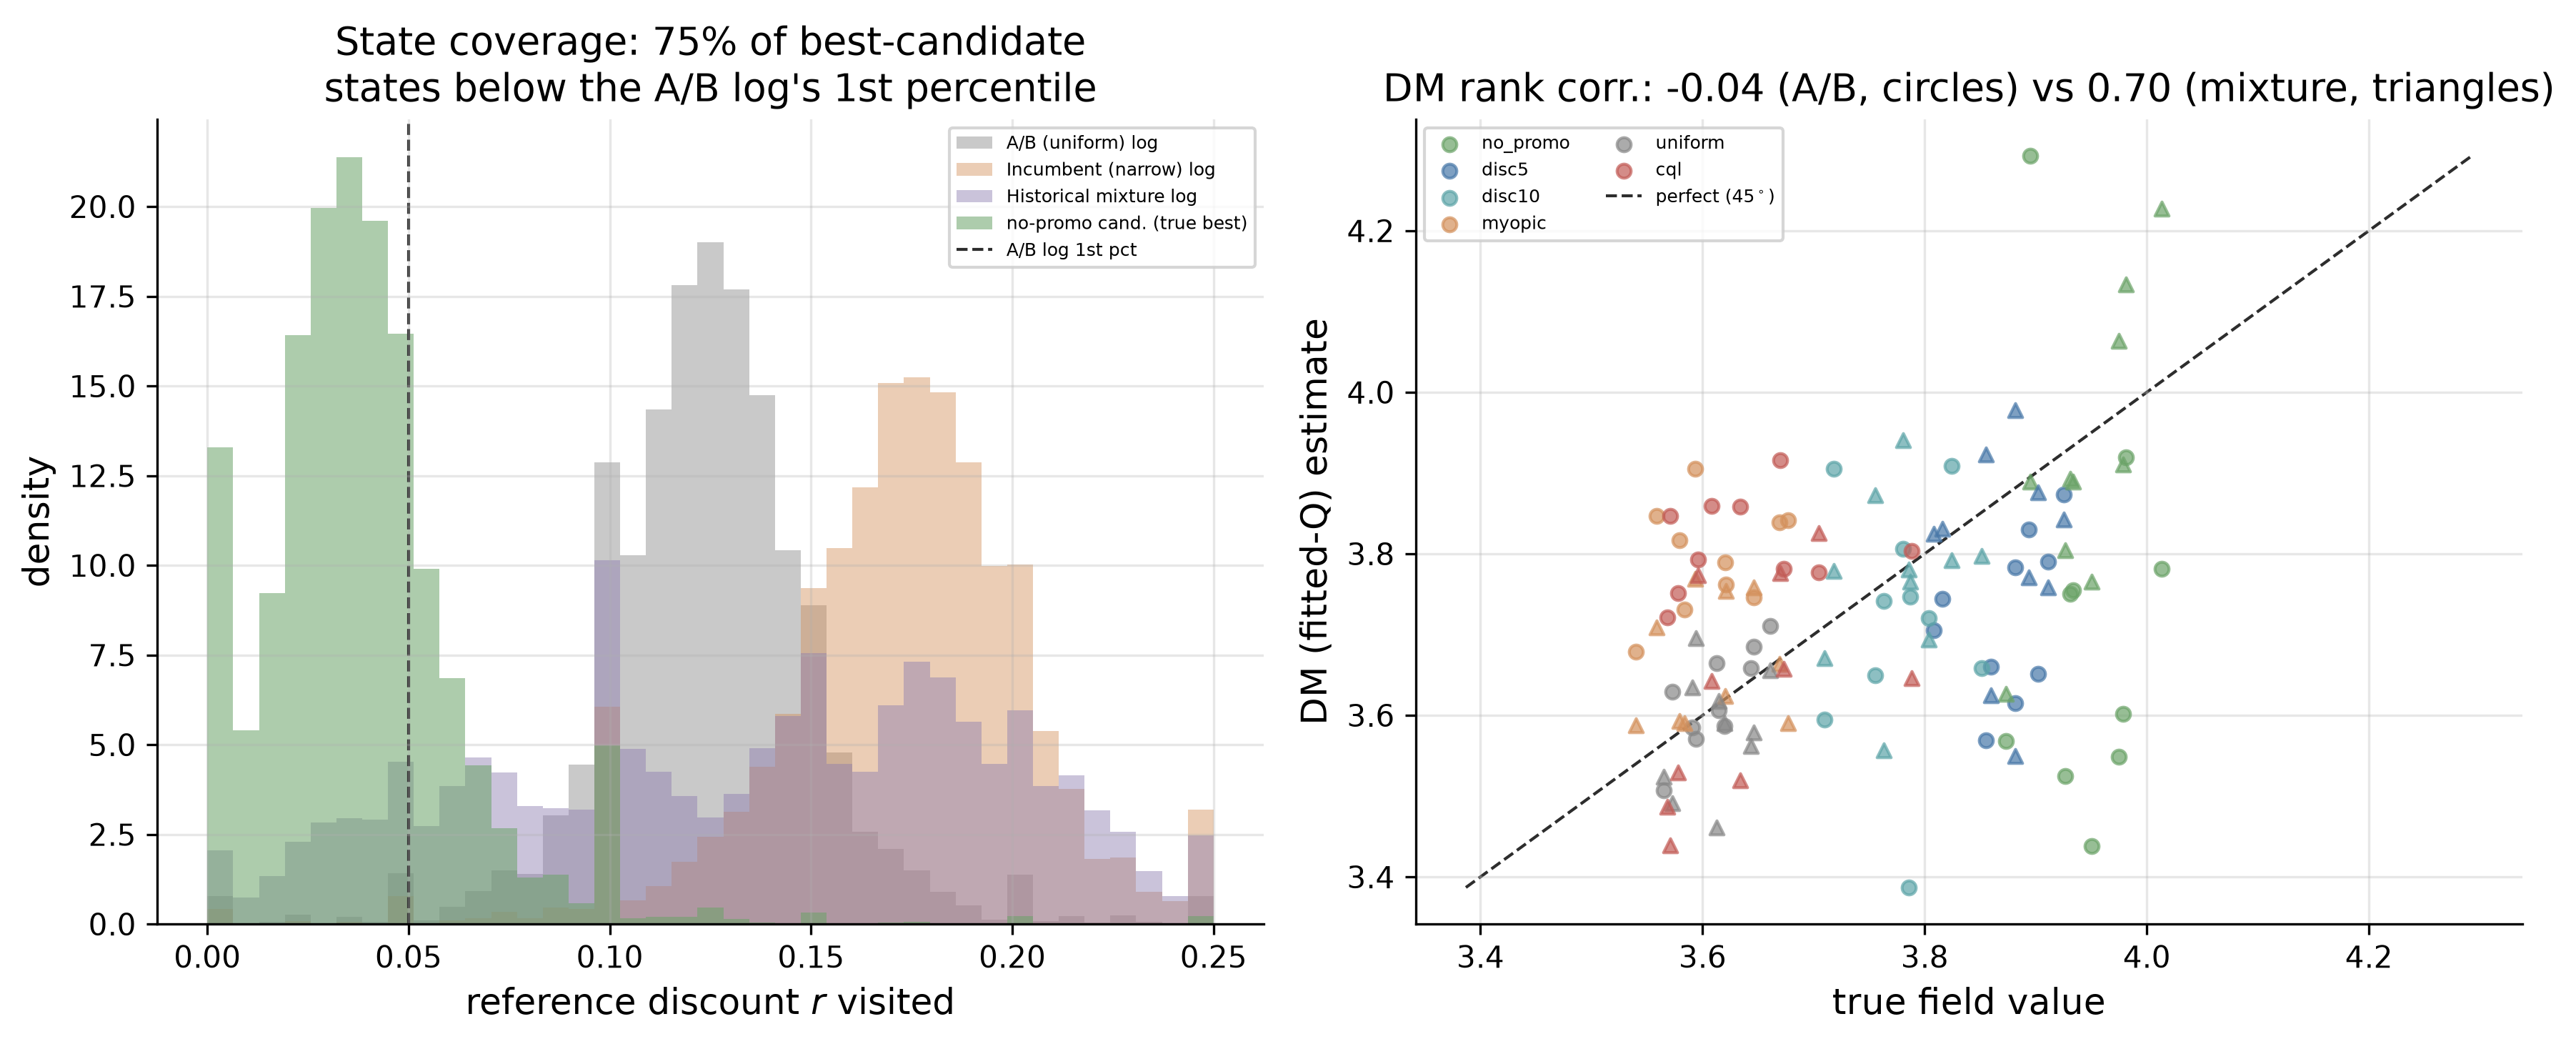
\includegraphics[width=\textwidth]{../ch13_field_deployments/sims/field_ope_reliability_mechanism.png}
\caption{Left: the market reference discount visited under the three logs and under the softened true-best (no-promo) candidate, with the dashed line at the first percentile of the A/B log. Right: the fitted-Q direct-method value estimate against the true field value under the A/B log (circles) and the historical-mixture log (triangles), pooled over \fieldopeseeds{} seeds, with the 45-degree reference line.}
\label{fig:field_ope}
\end{figure}

\begin{table}[t]
\centering
\small
\caption{Off-policy selection reliability of three estimators (direct method, DM; per-decision importance sampling, PDIS; doubly robust, DR) under three logging regimes, on the targeted-promotions MDP. Regret@1 is the value gap between the selected and the best deployment policy (reward units, lower is better); rank correlation is Spearman between estimated and true policy value (higher is better). Cells are mean (standard error) over 10 seeds.}
\label{tab:field_ope_reliability}
\begin{tabular}{lcccccc}
\toprule
 & \multicolumn{2}{c}{A/B (uniform)} & \multicolumn{2}{c}{Incumbent (narrow)} & \multicolumn{2}{c}{Historical mixture} \\
\cmidrule(lr){2-3}\cmidrule(lr){4-5}\cmidrule(lr){6-7}
Estimator & Regret@1 & Rank corr. & Regret@1 & Rank corr. & Regret@1 & Rank corr. \\
\midrule
DM & 0.210 (0.048) & -0.040 (0.116) & 0.246 (0.039) & -0.326 (0.136) & 0.038 (0.018) & 0.697 (0.053) \\
DR & 0.175 (0.046) & 0.051 (0.127) & 0.181 (0.043) & -0.166 (0.116) & 0.073 (0.033) & 0.423 (0.113) \\
PDIS & 0.265 (0.035) & -0.297 (0.110) & 0.326 (0.010) & -0.646 (0.083) & 0.268 (0.040) & 0.029 (0.103) \\
\bottomrule
\end{tabular}
\end{table}


\begin{table}[t]
\centering
\small
\caption{Per-candidate mechanism behind the reliability of Table~\ref{tab:field_ope_reliability}. True value is the Monte-Carlo on-policy field value; DM error is the fitted-Q direct-method estimate minus the true value (negative means under-valued); IS effective sample size is $(\sum w)^2/\sum w^2$ over the log's 500 trajectories. Rows are rank-ordered by true value; the true-best policy has the largest negative DM error and an effective sample size near one, while the uniform policy that generated the A/B log is the only one importance sampling can weight. Mean (standard error) over 10 seeds.}
\label{tab:field_ope_candidates}
\begin{tabular}{lccccc}
\toprule
 & & \multicolumn{2}{c}{DM error} & \multicolumn{2}{c}{IS eff.\ sample size} \\
\cmidrule(lr){3-4}\cmidrule(lr){5-6}
Candidate & True value & A/B & Obs. & A/B & Obs. \\
\midrule
No promo & 3.748 (0.009) & -0.634 (0.030) & -1.328 (0.098) & 1.509 (0.166) & 2.055 (0.255) \\
5\% discount & 3.680 (0.008) & -0.241 (0.024) & -0.954 (0.112) & 2.127 (0.456) & 1.653 (0.206) \\
10\% discount & 3.589 (0.009) & 0.154 (0.045) & -0.192 (0.066) & 1.908 (0.508) & 1.616 (0.172) \\
Uniform & 3.431 (0.007) & 0.256 (0.074) & -0.118 (0.113) & 500.000 (0.000) & 2.142 (0.421) \\
CQL (offline RL) & 3.417 (0.016) & 0.479 (0.041) & 0.300 (0.009) & 1.526 (0.205) & 3.641 (0.645) \\
Myopic incumbent & 3.399 (0.008) & 0.842 (0.020) & 0.250 (0.012) & 1.502 (0.233) & 3.773 (0.856) \\
\bottomrule
\end{tabular}
\end{table}


\subsection{Lessons from the Field}
\label{sec:field_lessons}

First, a deployed system gives reinforcement learning one small piece to control, not the whole problem. Meta's production bidding is the clearest case. The learner tunes the parameters of an existing bidding controller, the neural actor and critic are training machinery, and once training ends only the tuned controller is deployed, not the network. The method improves a trusted component in place, and that is what makes it safe to ship.

Second, the strongest cases have a constant stream of logged, repeated decisions. YouTube's recommender is the model here. Every recommendation is logged with the probability it was shown, the policy is trained from those logs with an off-policy correction, and a new version is tried on a small slice of live traffic before any wider launch. Dense logs and frequent feedback are what make offline learning, counterfactual checks, and cautious A/B testing possible, and settings without them rarely reach deployment.

Third, a conventional method stays in charge and reinforcement learning only feeds it. DiDi's dispatch keeps a matching problem that is solved every two seconds to assign drivers to orders, and the learner does not replace it but supplies the long-run value estimates that enter the matching weights. The systems that work do not ask a learned policy to rediscover operational knowledge the firm already has.

Fourth, how you check whether it worked depends on the domain. Tmall could not run an ordinary A/B test on price, because showing different customers different prices at the same time was not available to them, so the evaluation used difference-in-differences and comparisons across similar products instead. Digital products can randomize, pricing often cannot, physical systems alternate live periods under hard constraints, and a chip design is judged by hardware validation rather than an online metric.

Fifth, the public evidence comes in two kinds that are worth keeping apart. Some papers describe the whole integration. They state what the learner controlled, how it reached production, what guardrails and fallbacks surround it, and how the effect was measured. DiDi's dispatch and DeepMind's BCOOLER cooling controller are of this kind, and they are the ones a practitioner can actually learn from. Other papers run only on logged data or a simulator and still call the result ``real-world.'' Nevmyvaka's execution study, trained and tested on real order-book data through a historical backtest, is the archetype, and Wu's bidding paper reports only dataset splits while asserting industrial deployment. Evidence of the second kind shows that a method can fit logged data, not that it ran a live system, and the honest reading counts a deployment only when the source shows what was controlled in production.

A gap runs between reinforcement learning as it is studied and reinforcement learning as it is deployed. A benchmark rewards one policy that maximizes return inside a simulator, with the whole environment handed to the agent. A deployed system does close to the opposite. It gives the learner one narrow lever, a candidate slate at YouTube, the parameters of a bidding rule at Meta, a value estimate inside DiDi's matcher, a single quantization choice in one codec at MuZero-RC, and it leaves the surrounding controller, ranker, or optimizer in place. What ships is a small improvement to a system that already works, not an autonomous agent.

The gap also shows up in everything a deployment needs that a benchmark never scores. Logged data has to carry the probability each action was taken, and the learner has to correct for it, at YouTube, loosening the importance-weight cap alone moved a live metric by half a percent in the wrong direction. Actions have to pass through guardrails with a fallback to the incumbent controller when no safe action exists, as in BCOOLER. Training is kept offline and conservative because a mistake in a live auction or a live market is costly, so Meta learns its bidding policy from logs rather than exploring online. Around all of this sit shadow tests, switchback experiments, monitoring, and a retraining schedule. None of it is the learning algorithm, and all of it is why a system reaches production.

Finally, the bar is set by a strong incumbent, not a weak heuristic. A tuned base-stock policy already beats off-the-shelf deep RL on classic inventory problems, and DiDi's matcher and Meta's bidding rule were already good, so the reported gains are deliberately small and carefully measured, on the order of a percent or two. Clearing that bar reliably is hard, and an offline score is not enough to certify it. The simulation in Section~\ref{sec:field_ope_sim} makes the point concrete, since on a realistic pricing problem offline evaluation mis-ranks the candidate policies whenever the log's state occupancy fails to cover them, so a strong offline number can point at the wrong one. Taken together, this is why the confirmed list is short, why so many ``real-world'' papers stop at a simulator or a backtest, and why the field's honest claim is a narrow one. Reinforcement learning improves specific, well-instrumented parts of systems that were already running.

\subsection{When to Reach for Reinforcement Learning}
\label{sec:field_practitioner}

Before the deployment lessons of Section~\ref{sec:field_lessons} apply, a researcher deciding whether to try reinforcement learning in a firm faces a prior question, and it is worth answering first. The question is whether the firm's own actions move the state. When the context for each decision arrives on its own and the decision is scored in isolation, the problem is a contextual bandit or a supervised prediction, and the added machinery of full reinforcement learning buys nothing (Section~\ref{subsec:overlapping_terminology}). Reinforcement learning earns its cost only when today's action shapes tomorrow's world and the reward is delayed, when a discount today trains customers to wait for the next one, when a dispatch now leaves a region short later, or when a pricing rule changes how buyers behave (Section~\ref{sec:liu}). In the language of Section~\ref{section:language}, this is the control-culture move, taken when the dynamics are real and a myopic rule leaves long-run value unclaimed.

When the problem does have that structure, the deployed record marks out where reinforcement learning has actually paid off, and the profile is consistent. Decisions repeat at high volume and leave dense logs. The learner is given a narrow, well-defined lever inside a system the firm already runs, not the whole system. A strong incumbent is already in place, so the goal is a reliable small gain rather than a policy built from nothing. The logs record the probability of each action, so a policy can be both learned and checked from them. Mistakes are bounded and reversible, ideally behind guardrails with a fallback. And the outcome can be measured through some experiment the domain permits. The case catalog of Table~\ref{tab:field_case_inventory} is, in effect, the set of problems that met enough of these conditions.

Read in reverse, the same profile is a list of warning signs. Rare, one-shot, or low-volume decisions leave nothing to learn from. Logs without recorded action probabilities break both offline learning and its evaluation (Section~\ref{section:offline_rl}). A single catastrophic and irreversible mistake, with no guardrail to catch it, rules out live exploration. Where a myopic rule or a classical optimizer already captures the available value, reinforcement learning adds risk without adding return. The hardest warning to see is the last one, because an offline comparison can favor a policy that would fail in production, since a strong offline score can rank the wrong policy when the logs do not cover the states that policy would visit (Section~\ref{sec:field_ope_sim}).

A few cheap steps keep the effort small before it grows expensive. Start from the incumbent and look for where it leaves long-run value on the table, since that gap, not the algorithm, is the reason to reach for reinforcement learning at all. Prototype offline on the logs the firm already has, but treat the offline number with suspicion and check how much of the candidate policy's behavior those logs actually cover. Choose the narrowest lever that could plausibly move the target metric, and keep the current controller as the fallback. Decide the evaluation before building anything, because the domain, not the modeler, sets what is possible, a randomized test for a digital product, a difference-in-differences for prices, a switchback for a marketplace. Budget most of the work for the machinery around the policy, the logging, guardrails, monitoring, and retraining, which is where the deployed systems of Section~\ref{sec:field_lessons} were won or lost.

\subsection{The Shape of Deployed Reinforcement Learning}
\label{sec:field_shape}

It helps to see the confirmed record in one place. Table~\ref{tab:field_shape} lists, by domain, a representative deployed system, the reinforcement-learning method that actually ran, and the data or decision scale involved.

\begin{table}[t]
\centering
\footnotesize
\begin{tabularx}{\textwidth}{@{}>{\raggedright\arraybackslash}p{0.16\textwidth}>{\raggedright\arraybackslash}X>{\raggedright\arraybackslash}p{0.21\textwidth}>{\raggedright\arraybackslash}p{0.20\textwidth}@{}}
\toprule
Domain & Representative system & Method deployed & Data or decision scale \\
\midrule
Recommendation and ranking & YouTube top-$K$ \citep{Chen2019YouTubeTopK}; Taobao RL-LTV \citep{Ji2021RLLTV} & Off-policy REINFORCE; recurrent actor-critic & Web-scale logs; item-day episodes \\
Notification gating & Meta Horizon \citep{Gauci2019Horizon} & DQN send/drop & Production-scale logs \\
Bidding and auctions & Meta bidding \citep{Korenkevych2023MetaBidding}; Alibaba RTB \citep{Zhao2018SponsoredSearchRTB} & Offline RL tuning a base policy; robust-MDP DQN & $\sim$1.2B logged steps; $\sim$100M auctions per day \\
Dispatch and matching & DiDi \citep{SadeghiEshkevari2022DiDiScalable} & TD value inside a matching solver & Tens of millions of orders per day \\
Inventory & DeepStock \citep{Xie2026DeepStock} & Base-stock-regularized DDPG & More than 1M SKU-warehouse pairs \\
Video-codec rate control & MuZero-RC \citep{Mandhane2022MuZeroRC} & Model-based planning, policy served & Frame-level control on a live traffic slice \\
Chip floorplanning (design-time) & AlphaChip \citep{Mirhoseini2021GraphPlacement} & Graph policy-gradient & Transfer across prior chip blocks \\
LLM post-training (training-time) & InstructGPT \citep{ouyang2022training} & PPO against a reward model & Tens of thousands of labeled prompts \\
Building cooling (field trial) & BCOOLER \citep{Luo2022BCOOLER} & Constrained offline RL with fallback & Two commercial sites \\
\bottomrule
\end{tabularx}
\caption{The shape of confirmed field deployments: the domain, a representative system, the reinforcement-learning method that ran, and the data or decision scale. Firm types and evaluation practices are discussed in the text.}
\label{tab:field_shape}
\end{table}

Two regularities stand out. The data a deployment needs is domain-dependent and spans several orders of magnitude, from a two-building trial for BCOOLER, or tens of thousands of human-labeled prompts for InstructGPT, up to more than a billion logged time steps for Meta's bidding system and over a million stock-keeping-unit and warehouse pairs for DeepStock. The low-data cases survive only because their action is narrow and heavily constrained, while the high-volume cases are the recommendation, bidding, dispatch, and inventory systems where dense logs are a byproduct of ordinary operation. On method, two families carry almost all of the record. The first learns a value estimate and feeds it into a classical optimizer, as DiDi does with its matching solver and BCOOLER with its cooling controller. The second is DQN-style value-based control, used for notification gating, sponsored-search bidding, and price selection. Policy-gradient methods appear only when they are narrowed, by an off-policy correction at YouTube, by tuning a trusted base policy at Meta, or by optimizing against a reward model at OpenAI, and model-based planning appears once, at MuZero-RC. What is absent is as informative as what is present. No confirmed production system runs an unconstrained offline-RL policy such as conservative Q-learning, implicit Q-learning, or a model-based offline method as a standalone controller, and the one conservative-Q-learning case tunes the parameters of an existing bidding policy and deploys only those.

The domains that recur are a short list, recommendation, notification gating, bidding, dispatch, inventory, and codec control, and they share the shape above, a repeated high-volume decision wrapped around a system the firm already runs. Two cases sit outside that pattern and should be read as different evidence, since chip floorplanning is a design-time artifact that flows through ordinary hardware validation and RLHF is a training-time step whose product is a model rather than a live controller. The economically important spaces that are missing are missing for reasons the earlier conditions predict. Finance appears only as a historical backtest, healthcare not at all, robotics is set aside at the start of this chapter, and macroeconomic policy is nowhere, because those settings cannot cheaply or safely experiment on live decisions, often cannot randomize the real decision, and lack dense and fast feedback. The firms are correspondingly few. Almost every confirmed deployment comes from a handful of hyperscale platforms and frontier laboratories, among them Google, Meta, Alibaba, DiDi, OpenAI, and DeepMind, that hold all of the enabling conditions at once, the decision volume that makes a fractional gain worth capturing, the logging and off-policy evaluation, the engineering capacity, and an incumbent system to build around. The one non-technology operator in the record, a budget hotel chain, reached deployment only by simplifying the action to a single interpretable discount so that its managers would accept it.

A last difference is not about algorithms. The deployed record and the simulation literature measure different things. A benchmark reports return against a baseline on a fixed environment. A deployed system reports movement in the business quantity the firm is actually paid on, ViewTime at YouTube, gross merchandise value at Taobao, driver income at DiDi, revenue per available room in hotels, bitrate at fixed quality for MuZero-RC, inventory capital at DeepStock, and it reports that movement as a small, statistically significant change measured against a live control. The reported lifts are strikingly small, from a fraction of a percent to a few percent, and they are treated as real precisely because the denominator is enormous, so a fraction of a percent over fifty billion impressions or a million inventory pairs is a large absolute sum. The magnitude itself is a tell. The simulation and backtest cases in this chapter report gains of tens to over a hundred percent exactly because they never faced live control, which is the warning the simulation of Section~\ref{sec:field_ope_sim} makes precise, a large offline number is not evidence that a system will ship.

Around that headline number sit measurements a return curve never shows, and any one of them can decide whether a policy is deployable. Whether the offline evaluation can even be trusted becomes a tuned quantity, since YouTube's importance-weight cap is a hyperparameter whose relaxation costs half a percent of ViewTime, and Meta's platform runs a counterfactual evaluation as a required step before any launch. How to run the experiment is itself a design problem, because the real decision often cannot be randomized, so DiDi alternates by time slice and confirms the rollout with a difference-in-differences across cities, and Tmall compares against similar products because charging different prices at the same time is not allowed. Safety is a measured rate rather than an assumption, the frequency with which MuZero-RC overshoots its bitrate target, the rate at which BCOOLER hands control back to the incumbent controller, and the plain fact that an under-trained bidding agent can lose millions within hours. The operational budget is tracked on its own terms, a two-second serving path kept separate from a ten-second learning loop, a data lag under a day, a retraining cadence, and a monitor that compares this month against the year before. Long-run value, where it exists, is modeled explicitly, the lifetime value of a cold-start item at Taobao and the future value of a driver's location at DiDi, a horizon a one-step ranker misses by construction. None of these appear in a simulator's return, and together they are the difference between a method that wins a benchmark and one that runs a business.
